%!TEX root = thesis-kdyoung.tex

% \begin{savequote}%[45mm]
% If people do not believe that mathematics is simple, it is only because they do not realize how complicated life is.
% \qauthor{John von Neumann}
% \end{savequote}
\begin{savequote}%[45mm]
---Everything should be made as simple as possible, but not simpler.
\qauthor{Albert Einstein}
\end{savequote}

\chapter{Introduction}
\label{chap:intro}
Assembly lines are flow-based production systems widely used by
the manufacturing industry.
Designing these systems to meet the requirements set
by the industry gives rise to the Assembly Line
Balancing Problem (\albp{}).
An assembly line problem consists of a sequence
of \emph{stations} and a set of \emph{tasks}.
Stations are fixed points along the assembly
line which are operated by either human personnel
or autonomous machinery.
A workpiece is launched down the line and 
a subset of the tasks are performed on it at each station.
Once all required tasks are finished, the completed product
exits the assembly line.
% The construction of a single product is completed
% once all tasks have performed on it 
% To completely construct a single product
% the all tasks are performed along the line.
The workload of tasks must be divided among the stations
to optimize some performance measure,
while also respecting physical restrictions.
A standard example of such a restriction would be a
precedence relation, which can require
one task to be completed before another can begin
processing on the product.
The line itself is a mechanism used to
transport the products between stations;
most commonly the line is a conveyor belt.

There are two common objectives when designing an assembly
line, which each lead a distinct problem.
The first is called the type-1 problem and is concerned with
the design of a new assembly line where the production rate
of the product is predefined and the aim is to construct the line
with as few stations as possible, in-order to meet this demand.
The second problem, called type-2, considers the redesign of an existing
assembly line where the number of stations is fixed and the rate
of production is optimized.
The second case can arise when a manufacturing company alters their
production process or changes the products they offer.
Our thesis focuses on solving the type-2 problem.

The \emph{cycle time} of an assembly line defines the time each station
is given to perform its assigned tasks.
As such, finding the minimal possible cycle time 
is the primary aim when optimizing the production
rate of an assembly line.
Since all stations are connected by a single line,
the station with the largest workload will define the
overall cycle time of the line.
To achieve the minimal cycle time value,
we aim to balance the workload of the tasks
as evenly as possible among the stations.

The structure of the paper is as follows.
The remainder of Chapter \ref{chap:intro}
provides illustrative examples of the problem
and closes with some motivation.
In Chapter \ref{chap:theory} we detail a selection
of the relevant theory for our problem, spanning
the fields of Operations Research and Artificial Intelligence.
Chapter \ref{chap:mip} presents the mixed-integer
programs which were used to compare our
solution methodology against.
The construction of our logic-based Benders
decomposition is presented in Chapter \ref{chap:benders},
together with many possible modelling choices.
The results of our computational experiments are 
given in Chapter \ref{chap:exp}.
We conclude in Chapter \ref{chap:conc}
with some remarks on the performance of our
method and finally note a range of possible directions
for future research on this topic.

\section{Preliminaries and Examples}
\label{sec:intro:prelim}
The fundamental problem in this area is called the
Simple \albp{}, or \sab{}; we denote
the type-2 version by \sab{2}.
We now detail some straightforward examples
to illustrate how the workload
of an assembly line can be balanced.
In Example \ref{ex:intro:simple} we provide an instance
of the \sab{2} with a possible feasible solution and the optimal solution given
in Figures \ref{fig:intro:exSchedFeas} and \ref{fig:intro:exSchedOpt}
respectively. Note, that $t_i$ denotes the processing time of task $i$ and
$c$ denotes the cycle time of the assembly line.

\begin{example}\label{ex:intro:simple}
	Consider an instance of the problem with four tasks $T_1,\ldots,T_4$,
	and three stations $S_1,\ldots,S_3$,
	along the assembly line.
	The aim is to find an assignment of the tasks to the stations
	which minimizes the cycle time.
	This assignment must respect the precedence relations listed in Figure \ref{fig:intro:exPrec}, 
	\eg task $T_1$ must be completed before task $T_2$.
	The processing time of each task is included in Figure \ref{fig:intro:exPrec}
	next to each task.

	A feasible solution to this problem is given in Figure \ref{fig:intro:exSchedFeas},
	where the stations are spaced along the horizontal axis.
	Each station's workload begins at the horizontal axis and proceeds
	upward through time until all assigned tasks are completed.
	In this solution, the workload of $S_3$ is the largest
	and as such defines the cycle time as $t_3+t_4=2+9=11$.

	This feasible solution can be improved by moving task $T_3$ from station
	$S_3$ to $S_2$.
	For this assignment to remain feasible, $T_3$ must be processed
	after $T_2$, due to the precedence relations.
	This new assignment leads to the optimal solution listed in
	Figure \ref{fig:intro:exSchedOpt} with a cycle time of nine.	\qed
\end{example}

\begin{figure}[tpb]
	\centering
	\caption{Precedence graph}
	\vspace{2mm}
	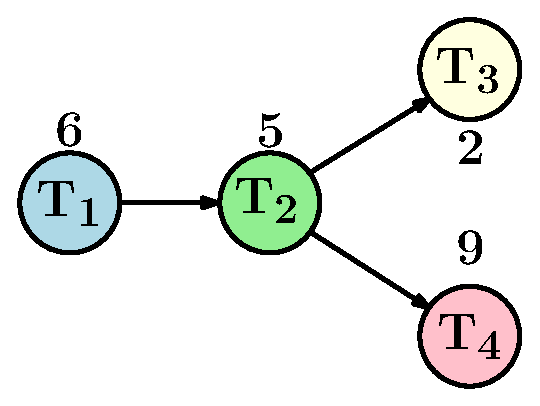
\includegraphics[width=0.45\textwidth]{images/precgraphSimple.eps}
	\label{fig:intro:exPrec}
\end{figure}

\begin{figure}[tpb]
	\centering
	\begin{minipage}{0.45\textwidth}
		\centering
		\caption{Feasible solution}
		\vspace{2mm}
		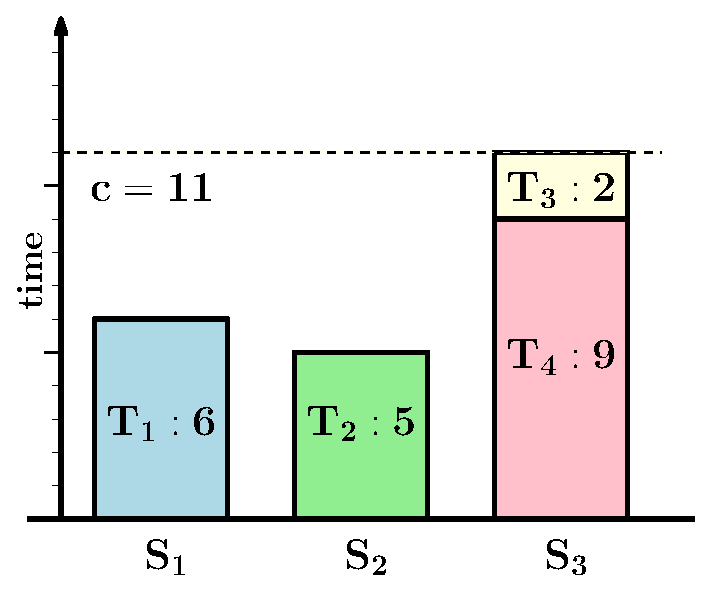
\includegraphics[width=\linewidth]{images/exSimpleFeas.eps}
		\label{fig:intro:exSchedFeas}
	\end{minipage}
	\hfill
	\begin{minipage}{0.45\textwidth}
		\centering
		\vfill
		\caption{Optimal solution}
		\vspace{2mm}
		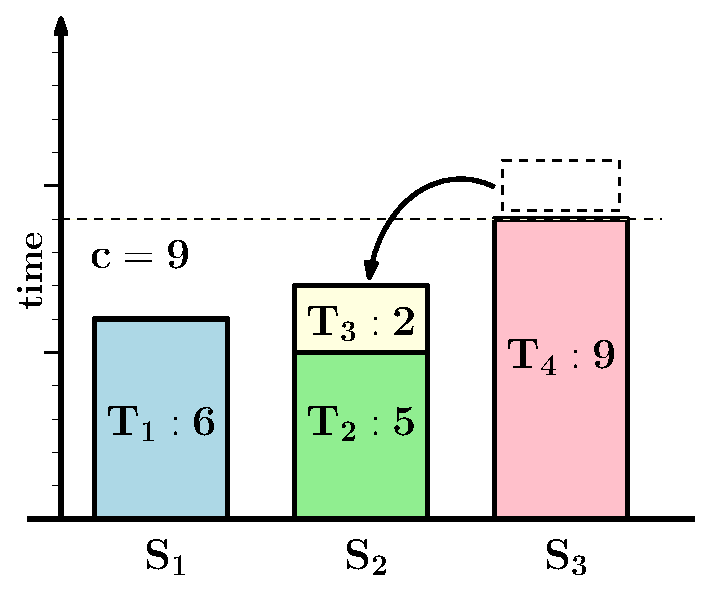
\includegraphics[width=\linewidth]{images/exSimpleOpt.eps}
		\label{fig:intro:exSchedOpt}
	\end{minipage}
\end{figure}

The variant of the \albp{} which we are concerned with adds the consideration
of sequence-dependent setup times between consecutive tasks
within a station's workload.
Theoretical approaches to the \albp{} usually assume that the assembly
line workers can decide on an arbitrary precedence-feasible sequence
to execute their assigned tasks, which will not affect the station's total
processing time.
However, in practice there can be non-trivial setup costs, due
to walking times or tool changes, which can account for a considerable amount
of a station's processing time.
Adding this consideration to the problem
leads to a scheduling problem arising within each station.
This variant of the problem is called the SetUp Assembly Line Balancing and
Scheduling Problem (\sua{}).

To realistically model the setup costs that occur
in assembly lines, two types of setups are introduced;
\emph{forward} and \emph{backward} setups.
A forward setup time, denoted by $\phi$, occurs between two consecutive
tasks within a station's task sequence if both tasks
are performed on the same product.
Whereas a backward setup time, denoted by $\beta$, occurs between the last task
performed on a product and the first task performed on
the next product along the line.

\begin{figure}[tpb]
	\centering
	\caption{Cyclic task sequence of a station (adapted from \cite{Scholl2013})}
	\vspace{2mm}
	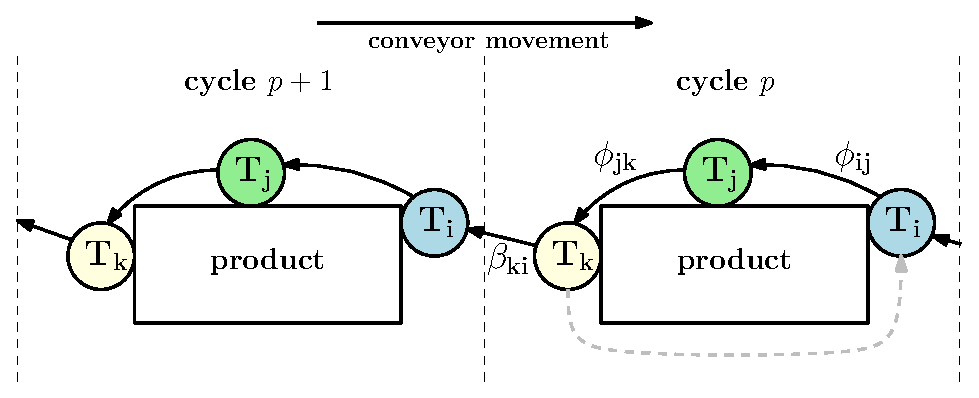
\includegraphics[width=0.8\textwidth]{images/IntroForwBackSetupEx.eps}
	\label{fig:intro:forwBackDifference}
\end{figure}

To see how these setups are differentiated, 
Figure \ref{fig:intro:forwBackDifference} depicts the sequence of tasks 
$T_i,\:T_j,\:T_k$ which are performed in a cyclic manner on consecutive
products.
The execution of tasks proceeds chronologically from right to left,
\ie $T_1$ is the first task performed in cycle $p$.
Forward setups arise between consecutive tasks operating
on the same product.
A backward setup cost is incurred between the last
task of cycle $p$ and the first task of the next cycle, $p+1$.
Each cycle begins at time zero with the execution of task $T_i$
taking $t_i$ time units to process.
Then after performing the forward setups $\phi_{ij}$ and $\phi_{jk}$
together with processing times $t_j$ and $t_k$,
the station operator must perform the necessary backward
setup operation before moving to the next
workpiece along the line. 
Thus, when including this backward setup time $\beta_{ki}$,
the following condition must be satisfied to have a 
feasible cycle time
$t_i+\phi_{ij}+t_j+\phi_{jk}+t_k+\beta_{ki} \leq c$.
In Figure \ref{fig:intro:forwBackDifference}, the gray arrow  from $T_k$ to $T_i$ implies
the cyclic nature of the sequence.

% Example \ref{ex:intro:simpleSetup} alters the previous
% example into an instance of the \sua{2}.

\begin{example}\label{ex:intro:simpleSetup}
	Again consider the instance from Example \ref{ex:intro:simple},
	but now with sequence-dependent setup times
	between tasks.
	The arrays of forward and backward setup costs
	can be found in Tables \ref{tab:intro:forwSetupTimes}
	and \ref{tab:intro:backSetupTimes} respectively.
	Note, that some of the entries in these arrays are
	omitted as the corresponding sequence of tasks is not 
	possible due to the precedence relations or
	logical restrictions.

	The previous optimal solution is amended
	to include the required setup costs and is given in Figure 
	\ref{fig:intro:exSchedSetupFeas}.
	Note that the setup cost of any task to itself is 
	defined as zero.
	% This results in a large forward setup, $\phi_{23}$,
	% occurring on station $S_2$.
	To reach the optimal solution we must now consider
	the sequence of tasks within each station.

	By moving task $T_3$ to station $S_3$ and considering
	the sequencing of $T_3$ and $T_4$, we find the optimal
	solution to this problem, given in Figure \ref{fig:intro:exSchedSetupOpt}.
	The optimal cycle time is 13 in this case.	\qed
\end{example}

\begin{table}[tpb]
	\centering
	\begin{minipage}{0.45\textwidth}
		\def\arraystretch{1.1}
		\centering
		\caption{Forward setup times}
		\vspace{2mm}
		\begin{tabular}{lllll}
			\toprule
			$\phi$ & $T_1$ & $T_2$ & $T_3$ & $T_4$ \\\midrule\midrule
			$T_1$ & -- & 3 & 3 & 3 \\
			$T_2$ & -- & -- & 2 & 3 \\
			$T_3$ & -- & -- & -- & 1 \\
			$T_4$ & -- & -- & 2 & -- \\
			\bottomrule
		\end{tabular}
		\label{tab:intro:forwSetupTimes}
	\end{minipage}
	\hfill
	\begin{minipage}{0.45\textwidth}
		\def\arraystretch{1.1}
		\centering
		\caption{Backward setup times}
		\vspace{2mm}
		\begin{tabular}{lllll}
			\toprule
			$\beta$ & $T_1$ & $T_2$ & $T_3$ & $T_4$ \\\midrule\midrule
			$T_1$ & 0 & -- & -- & -- \\
			$T_2$ & 3 & 0 & -- & -- \\
			$T_3$ & 3 & 5 & 0 & 3 \\
			$T_4$ & 3 & 3 & 1 & 0 \\
			\bottomrule
		\end{tabular}
		\label{tab:intro:backSetupTimes}
	\end{minipage}
\end{table}

\begin{figure}[tpb]
	\centering
	\begin{minipage}{0.47\textwidth}
		\centering
		\caption{Feasible solution with setup}
		\vspace{2mm}
		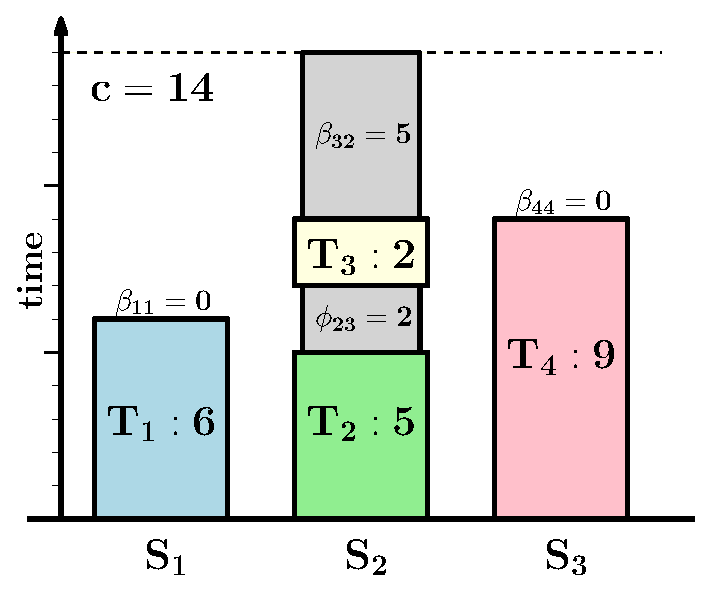
\includegraphics[width=\linewidth]{images/exSimpleSetupFeas.eps}
		\label{fig:intro:exSchedSetupFeas}
	\end{minipage}
	\hfill
	\begin{minipage}{0.47\textwidth}
		\centering
		\caption{Optimal solution with setup}
		\vspace{2mm}
		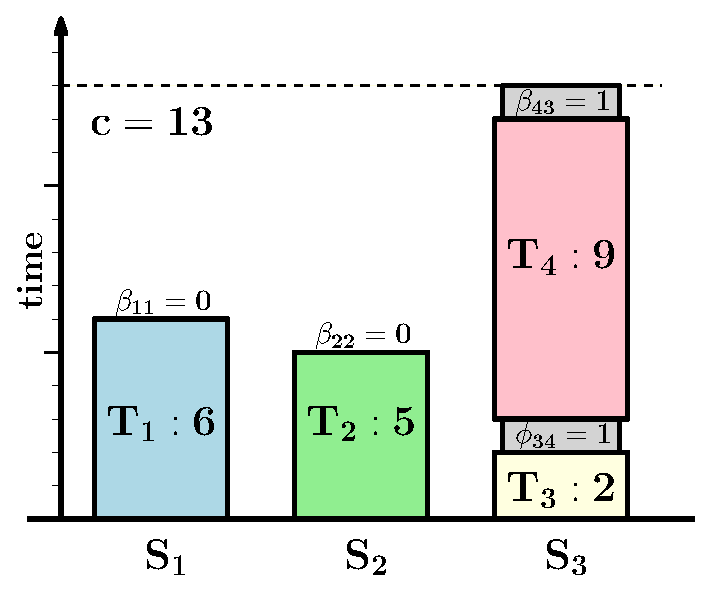
\includegraphics[width=\linewidth]{images/exSimpleSetupOpt.eps}
		\label{fig:intro:exSchedSetupOpt}
	\end{minipage}
\end{figure}

\section{Motivation}
\label{sec:intro:motiv}
In this section we provide motivation for why the \albp{}
with setup costs
is an important problem to be solved and why the approach we
chose to utilize is well-suited to the problem.

\subsection{Why the SUALBSP?}
Assembly lines were originally designed for the production
of a single type of product in high volumes.
Although, assembly lines able to produce only a single
product are not suitable for consumer-centric markets, 
where there is a need to tailor the products
more closely to the user's needs.
Sequence-dependent setup times are commonly considered
in job shop scheduling problems and a range of other
production problems (\cf \cite{Allahverdi2008a,Allahverdi2008b,Allahverdi2015}).
In those problems, the setup times arise because the products
are typically assumed to be highly diverse,
leading to additional configuration effort being required
between any two tasks.
In the context of operational planning of assembly lines,
sequence-dependent setup times have been sparsely
considered by the literature.
\authciteb{Scholl2013} list a number of possible
practical settings where setup times between tasks should not
be taken as negligible. Some include the following:
\begin{itemize}
	\item In automotive assembly lines where large workpieces (vehicles)
	need to be constructed, work can be performed at numerous
	mounting positions on the item.
	The size of the car body can result in walking distances
	between mounting positions being non-trivial.
	Thus, the preparation time (setup) can 
	be a critical aspect when sequencing the required tasks.
	\item Fixed material containers can be placed along the moving 
	conveyor system to allow workers to collect parts or tools needed.
	Further to walking times between these containers and the workpiece,
	the time taken to retrieve what is required from the container
	must also be accounted for.
	At a major German car manufacturer, these times contributed $10-15\%$
	of the total cycle time \cite{Scholl2013}.
	\item Specific tools are often required to perform a task.
	If consecutive tasks need different tools for their
	execution a tool-change between tasks will be necessary.
	Robotic assemblers used to perform the tasks of a station
	can be built to be highly flexible in the types of tasks
	they can perform.
	However, this flexibility can mean that numerous tool changes
	are required to switch from one task to another
	in a sequence.
	Thus, these sequence-dependent setup costs from tool-changes
	are typical in robotic assembly lines.
\end{itemize}
Consequently, accurately modelling the setup costs incurred
can be an important aspect when balancing an assembly line.

In practice, setup times are accounted for in simpler ways, such as
using an approximation or incorporating the setup time
into the task's processing time.
\citeauthor{Scholl2013} note that by using such approximations
``the planning team need to strike a fragile balance between an underestimation
of setups, which lead to infeasible line balances, and an overestimation
of setups, which leads to an allocation of excessive resources.''
The procedure used to estimate the cost of setups
can be time consuming and is prone to getting stuck in sub-optimal solutions.

For these reasons we feel that further research into the 
effect of setup times on the \albp{} is of interest to the
academic community and the manufacturing industry.

\subsection{Why Benders Decomposition?}
Benders decomposition is a well-known approach
to optimization problems.
It is naturally suited
to problems where the decisions can be separated into
two distinct sets.
Advances in the past few decades to the theory of
this method has broadened its applicability to a 
wider array of problems.
In our case, a solution to the \sua{2} can naturally
be divided into the assignment portion, which
assigns each task to a station, and the scheduling
portion, which decides on the time that each task
begins execution within a station.

We can view this separation of concerns in the following
way.
The manager of an assembly line needs a new item
to be put into production and so assigns the required
set of tasks to the stations along the line.
When calculating the line's cycle time the manager only estimates the setup times
within each station.
Each station operator must then decide if a possible sequencing
of their assigned tasks exists which can respect the manager's cycle time;
or if a precedence-feasible sequence exists at all.
% The worker at each station must then decide if there exists
% a possible sequencing of their assigned tasks which can
% respect the manager's cycle time; or if there a
% precedence-feasible sequence exists at all.
If at least one worker cannot find a feasible task-sequence
that respects the manager's cycle time
estimate, then a revision
may need to be made to the assignment of tasks.
The give-and-take between the assignment and scheduling portions
continues until a mutually satisfactory solution is found.
This informal process of communicating information between
the station workers and the assembly line manager could be time
consuming and not guarantee optimality.

The informal feedback loop between the two halves of the
decision problem suggests that Benders decomposition could be
employed to mimic this process.
The decision making process can naturally be divided
into a master problem, which assigns the tasks
to the stations along the line,
and several independent scheduling problems.
In total, there is a sub-problem
for each of the $m$ stations, which needs to
decide the exact execution time of all tasks
that station has been assigned.
Each sub-problem is similar to the asymmetric
Travelling Salesperson Problem (TSP)
with some forbidden paths due to the precedence
relations.
With this interpretation, the tasks are viewed as the 
cities and distances between them are the setup times.
To complete the iterative loop, the sub-problems
relay their information back to the master as
Benders cuts and the assignment problem is re-optimized.
In the words of J. N. Hooker,
``the Benders cuts added to the master problem are
the mathematical equivalent of telephone calls''
from the station workers to the line manager \cite{Hooker2007}.

The reader may be familiar with the classical version
of the Benders decomposition method due to the 
work of \authciteb{Benders1962} and \authciteb{Geoffrion1972},
however for the \sua{}, this approach is inappropriate.
Due to the sub-problems being highly-combinatorial discrete scheduling
problems, formulating them as a linear or non-linear program
will not be practical.
We instead explore how the more general method of \emph{logic-based}
Benders decomposition can be used to solve the \sua{2}.

By employing this approach we are able to exploit the comparative
advantages of multiple solving technologies to tackle each
portion of the problem.
Mixed-Integer Programs (MIPs) are well-suited to the assignment
problem of the master and Constraint Programming (CP), from 
the Computer Science discipline, is an effective solving technology
for scheduling problems.

\section{Problem Definition}
\label{sec:intro:probDef}
Here we present the core notation that will be used for the
remainder of the thesis.
Along the conveyor belt of the assembly line
there are \emph{work stations} $K=\{1,2,\ldots,m\}$.
Workpieces (or products/items) move down the 
conveyor belt from station to station.
A workpiece remains at each station for 
one cycle, which has a duration given by the \emph{cycle time}.
The objective of the \albp{} is to optimally partition
the total work required among the stations with respect to
a performance measure.

The work required to complete a single piece is separated into
a set of \emph{non-preemptive tasks} $V=\{1,2,\ldots,n\}$,
each with a discrete processing time $t_i$.
Physical and technical conditions impose a set of 
\emph{precedence relations} $E\subseteq V\times V$,
which prevent some non-allowed task orderings from occurring.
If we consider the graph $G=(V,E)$ with tasks as the vertex set
and directed edges defined by the precedence relations,
then $G$ is a directed acyclic graph (DAG).	
Without loss of generality, we may assume that the vertices
are numbered topologically so that the following holds:
$(i,j) \notin E$ if $i>j$.

Between each pair of tasks, discrete
\emph{forward} and \emph{backward setup} times
are predefined.
We denote the forward setup time between $i$ and $j$
by $\phi_{ij}$ and the backward setup time
by $\beta_{ij}$.
When $i=j$, the forward setup time is undefined
as a task can never follow itself in a station's
forward work load.
The backward setup $\beta_{ii}$, \ie the setup cost
of a task to itself, is defined as zero.

To fully specify a feasible solution to the \sua{2},
one must give the following:
an assignment of tasks to the stations
and the execution time window of each task within
its assigned station.
From this specification, the cycle time is calculated by
the total processing time of the station with the
largest workload.

